\documentclass{article}
\usepackage{hyperref}
\usepackage{float}
\usepackage{graphicx}
\graphicspath{ {./images/} }
\begin{document}

\title{Car Accident Severity Prediction}
\author{Sudipto Ghosh}
\date{September 13, 2020}
\maketitle

\section{Introduction}

\subsection{Background}

The Open Data Program makes the data generated by the City of Seattle has been openly available to the public for the purpose of increasing the quality of life for the residents, increasing transparency, accountability and comparability, promoting economic development and research, and improving internal performance management.

The Traffic Records Group, Traffic Management Division, Seattle Department of Transportation, provides data for all collisions and crashes that have occurred in the state from 2004 to the present day. The data is updated weekly and can be found at the Seattle Open GeoData Portal\footnote[1]{\href{https://data-seattlecitygis.opendata.arcgis.com/}{https://data-seattlecitygis.opendata.arcgis.com/}}.

\subsection{Motivation}

We can exploit this data to extract vital features that would enable us to end up with a good model that would enable the prediction of the severity of future accidents that take place in the state. This would further enable the Department of Transportation to prioritise their SOPs and channel their energy to ensure that fewer fatalities result in automobile collisions.

\section{Data}

\subsection{Data Understanding}

The dataset is available as comma-separated values (CSV) files, KML files, and ESRI shapefiles that can be downloaded from the Seattle Open GeoData Portal. The data is also available from RESTful API services in formats such as GeoJSON. We download the dataset to our project directory and take a look at the data types and the dimensionality of the data. We could see that the dataset contains 221,389 records and 40 fields.

The metadata of the dataset can be found from the website of the Seattle Department of Transportation\footnote[2]{\href{https://www.seattle.gov/Documents/Departments/SDOT/GIS/Collisions\_OD.pdf}{https://www.seattle.gov/Documents/Departments/SDOT/GIS/Collisions\_OD.pdf}}.

On reading the dataset summary, we can determine the description of each of the fields and their possible values. The data contains several categorical fields and corresponding descriptions which could help us in further analysis. We made an attempt at understanding the data in terms of the fields that we shall take into account for later stages of model building.

\begin{table}
  \centering
  \begin{tabular}{|c | c|}
  \hline
  Field Name & Description\\
  \hline
  X & Longitude (in degree decimal)\\
  Y & Latitude (in degree decimal)\\
  OBJECTID & ESRI unique identifier\\
  INCKEY & Unique key for the incident\\
  COLDETKEY & Secondary key for the incident\\
  REPORTNO & NA\\
  STATUS & NA\\
  ADDRTYPE & Collision address type: [Alley, Block, Intersection]\\
  INTKEY & Key to the intersection associated with a collision \\
  LOCATION & Description of the general location of the collision \\
  EXCEPTRSNCODE & NA\\
  EXCEPTRSNDESC & NA\\
  SEVERITYCODE & Code corresponding to the severity of the collision\\
  SEVERITYDESC & Detailed description of the severity of the collision\\
  COLLISIONTYPE & Collision type\\
  PERSONCOUNT & Total number of people involved in the collision\\
  PEDCOUNT & Number of pedestrians involved in the collision\\
  PEDCYLCOUNT & Number of bicycles involved in the collision\\
  VEHCOUNT & Number of vehicles involved in the collision\\
  INJURIES & Number of total injuries in the collision\\
  SERIOUSINJURIES & Number of serious injuries in the collision\\
  FATALITIES & Number of fatalities in the collision\\
  INCDATE & Date of the incident\\
  INCDTTM & Time of the incident\\
  JUNCTIONTYPE & Category of junction where collision took place\\
  SDOT\_COLCODE & Code given to the collision by SDOT\\
  SDOT\_COLDESC & Description of the collision by SDOT\\
  INATTENTIONIND & Whether collision was due to inattention\\
  UNDERINFL & Whether under the influence of drugs or alcohol\\
  WEATHER & Description of the weather conditions\\
  ROADCOND & Condition of the road during the collision\\
  LIGHTCOND & Light conditions during the collision\\
  PEDROWNOTGRNT & Whether pedestrian right of way was not granted\\
  SDOTCOLNUM & Number given to the collision by SDOT\\
  SPEEDING & Whether speeding was a factor in the collision\\
  ST\_COLCODE & Code provided by the state for the collision\\
  ST\_COLDESC & Description according to the state’s coding scheme\\
  SEGLANEKEY & Key for lane segment where the collision occurred\\
  CROSSWALKKEY & Key for crosswalk where the collision occurred\\
  HITPARKEDCAR & Whether collision involved hitting a parked car\\
  \hline
  \end{tabular}
  \caption{Fields in the Dataset}\label{fields}
\end{table}

As the dataset has possibly been sourced from a database table, several unique identifiers and spatial features are present in the database which may be irrelevant in further statistical analysis. These fields are OBJECTID, INCKEY, COLDETKEY, INTKEY, SEGLANEKEY, CROSSWALKKEY, and REPORTNO. Other fields such as EXCEPTRSNCODE, SDOT\_COLCODE, SDOTCOLNUM and LOCATION and their corresponding descriptions (if any) are categorical but have a large number of distinct values that shall not be that much useful for analysis. The INCDATE and INCDTTM denote the date and the time of the incident but may not be of use in further analyses. The data needs to be pre-processed.

\subsection{Statistical Insights}

We used the Matplotlib and Seaborn libraries to visualize the distributions in the dataset. We plotted various countplots, which are histograms across categorical, instead of quantitative, variables, for the distribution of WEATHER, ROADCOND, and LIGHTCOND fields.

\begin{figure}[H]
  \centering
  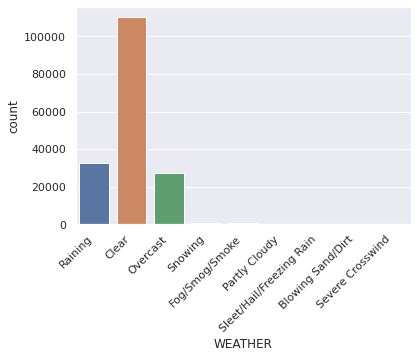
\includegraphics[scale=0.4]{weather.png}
  \caption{Weather Distribution}
\end{figure}

\begin{figure}[H]
  \centering
  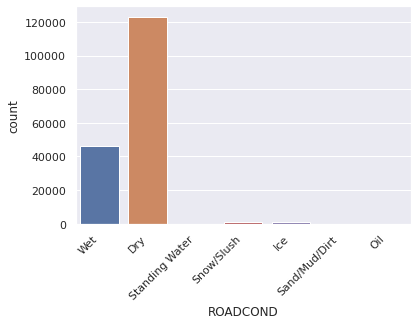
\includegraphics[scale=0.4]{roadcond.png}
  \caption{Road Condition Distribution}
\end{figure}

\begin{figure}[H]
  \centering
  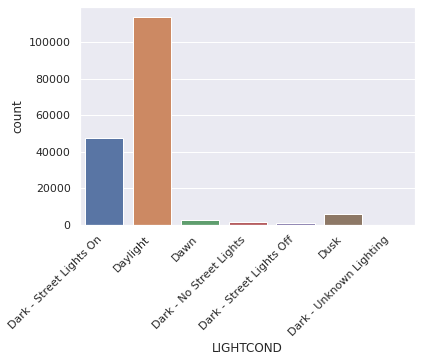
\includegraphics[scale=0.4]{lightcond.png}
  \caption{Light Condition Distribution}
\end{figure}

\begin{figure}[H]
  \centering
  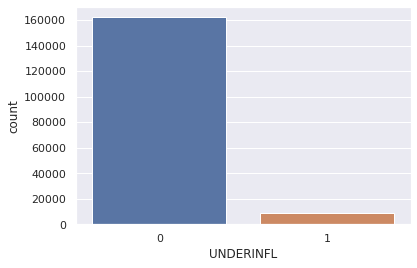
\includegraphics[scale=0.4]{underinfl.png}
  \caption{Under Influence Distribution}
\end{figure}

We also used scatter plots to visualize the relationship between various fields such as PERSONCOUNT, VEHCOUNT, INJURIES, and PEDCOUNT.

\begin{figure}[H]
  \centering
  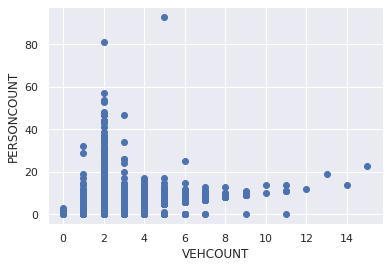
\includegraphics[scale=0.4]{vehperson.png}
  \caption{Vehicle Count v/s Person Count}
\end{figure}

\begin{figure}[H]
  \centering
  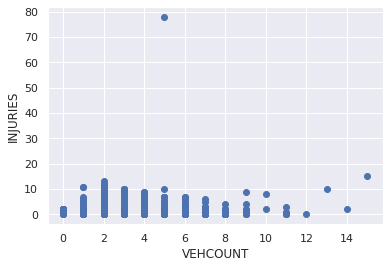
\includegraphics[scale=0.4]{vehinjuries.png}
  \caption{Vehicle Count v/s Injuries}
\end{figure}

\begin{figure}[H]
  \centering
  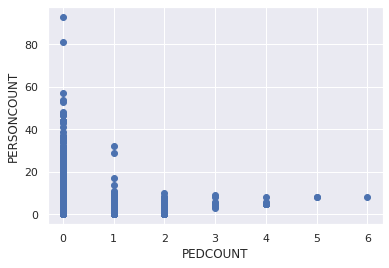
\includegraphics[scale=0.4]{pedperson.png}
  \caption{Pedestrian Count v/s Person Count}
\end{figure}

Correlation is a statistical technique that can show whether and how strongly pairs of variables are related. Finding the correlation among the features of the dataset helps understand the data better. For example, in the plots given below, it can be observed that some features have a strong positive / negative correlation while most of them have weak / no correlation.

\begin{figure}[H]
  \centering
  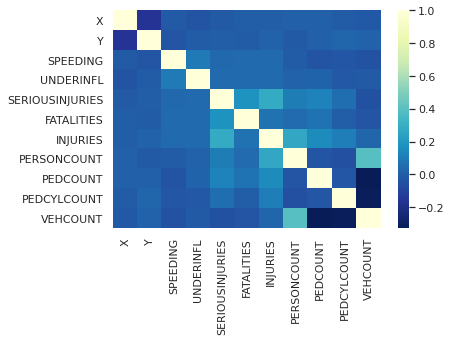
\includegraphics[scale=0.65]{heat1.png}
  \caption{Correlation Plot before Encoding}
\end{figure}

\begin{figure}[H]
  \centering
  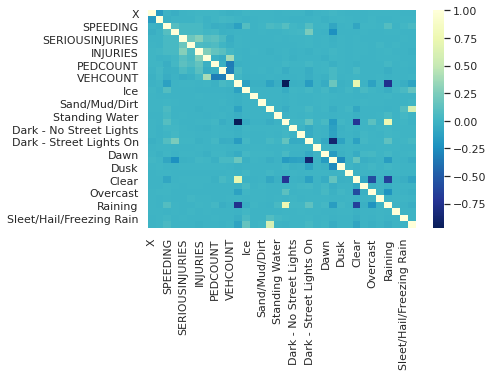
\includegraphics[scale=0.65]{heat2.png}
  \caption{Correlation Plot after Encoding}
\end{figure}

\section{Methodology}

\subsection{Data Pre-processing}

We use Pandas and NumPy for this task. After removing the blanks and duplicated records, certain fields were chosen and others were dropped. Data inconsistencies were also fixed. A heatmap was used to have a high-level overview of blanks in the dataset. We chose the following fields for the analysis:

\begin{figure}[H]
  \centering
  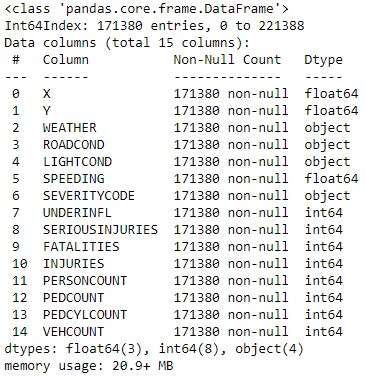
\includegraphics[scale=0.65]{finalfields.jpg}
\end{figure}

\begin{figure}[H]
  \centering
  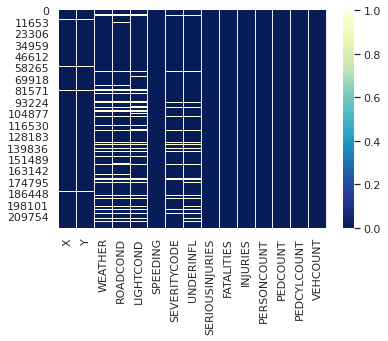
\includegraphics[scale=0.6]{blanks1.png}
  \caption{Dataset before Data Cleaning}
\end{figure}

\begin{figure}[H]
  \centering
  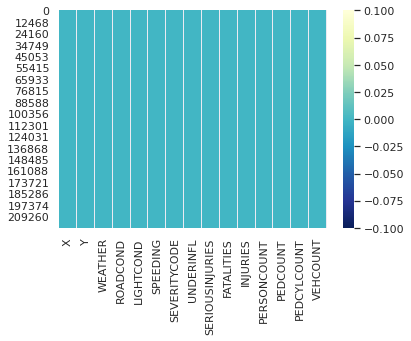
\includegraphics[scale=0.6]{blanks2.png}
  \caption{Dataset after Data Cleaning}
\end{figure}

Datasets \emph{x} and \emph{y} are constructed. The set \emph{x} contains all the training examples and y contains all the labels. Feature scaling of data is done to normalize the data in a dataset to a specific range. After normalization, they are split into \emph{x\_train},\emph{ y\_train}, \emph{x\_test}, and \emph{y\_test}. The first two sets shall be used for training and the last two shall be used for testing. Upon choosing a suitable split ratio, 80\% of data is used for training and 20\% of is used for testing.

\subsection{Modelling and Evaluation}

We use SciKit-Learn and TensorFlow for this task.

\subsubsection{Decision Tree Classifier}

Decision Tree makes decision with tree-like model. It splits the sample into two or more homogenous sets (leaves) based on the most significant differentiators in the input variables. To choose a differentiator (predictor), the algorithm considers all features and does a binary split on them (for categorical data, split by category; for continuous, pick a cut-off threshold). It will then choose the one with the least cost (i.e. highest accuracy), and repeats recursively, until it successfully splits the data in all leaves (or reaches the maximum depth).

Information gain for a decision tree classifier can be calculated either using the Gini Index measure or the Entropy measure, whichever gives a greater gain. A hyper parameter Decision Tree Classifier was used to decide which tree to use, DTC using entropy had greater information gain; hence it was used for this classification problem.

\begin{figure}[h]
  \centering
  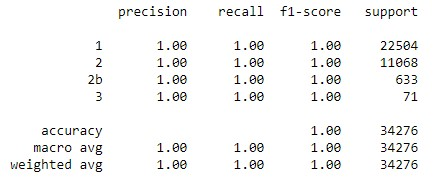
\includegraphics[scale=0.8]{dtcreport.jpg}
  \caption{Classification Report for Decision Tree Classifier}
\end{figure}

\subsubsection{Random Forest Classifier}

Random Forest Classifier is an ensemble\footnote{algorithms which combines more than one algorithms of same or different kind for classifying objects} tree-based learning algorithm. RFC is a set of decision trees from randomly selected subset of training set. It aggregates the votes from different decision trees to decide the final class of the test object. Used for both classification and regression.

Similar to DTC, RFC requires an input that specifies a measure that is to be used for classification, along with that a value for the number of estimators (number of decision trees) is required. A hyperparameter was used to determine the best choices for the above mentioned parameters. RFC with 75 DT’s using entropy as the measure gave the best accuracy when trained and tested on pre-processed accident severity dataset.

\begin{figure}[h]
  \centering
  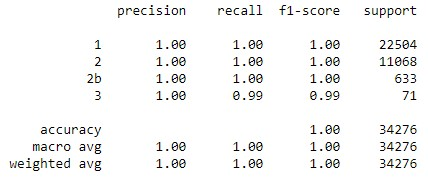
\includegraphics[scale=0.8]{rfcreport.jpg}
  \caption{Classification Report for Random Forest Classifier}
\end{figure}

\subsubsection{Logistic Regression Classifier}

Logistic Regression is a classifier that estimates discrete values (binary values like 0/1, yes/no, true/false) based on a given set of an independent variables. It basically predicts the probability of occurrence of an event by fitting data to a logistic function. Hence it is also known as logistic regression. The values obtained would always lie within 0 and 1 since it predicts the probability. The chosen dataset has more than two target categories in terms of the accident severity code assigned, one-vs-one (OvO) strategy is employed.

\begin{figure}[h]
  \centering
  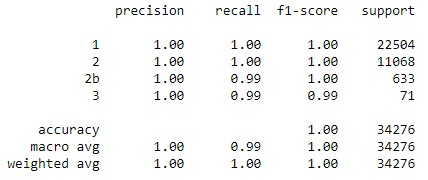
\includegraphics[scale=0.8]{logregreport.jpg}
  \caption{Classification Report for Logistic Regression Classifier}
\end{figure}

\subsubsection{Artificial Neural Network}

Neural networks can be used to capture non-linearity between features. We have used a Sequential ANN where there are 2 hidden layers. The \emph{relu} and \emph{sigmoid} activation functions are used. The loss function that is used is \emph{categorical\_crossentropy} as the target is integer-coded. As neural networks are prone to over-fitting, we plotted the Loss and Accuracy curves for the training and validation sets to make sure the model is not over-fitted.

\begin{figure}[H]
  \centering
  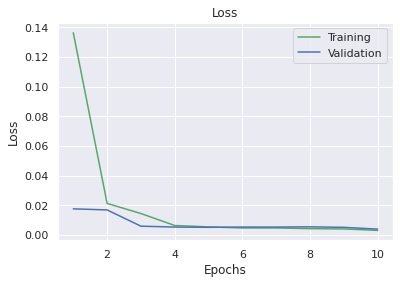
\includegraphics[scale=0.75]{lossevo.png}
  \caption{Loss Curve for Artificial Neural Network}
\end{figure}

\begin{figure}[H]
  \centering
  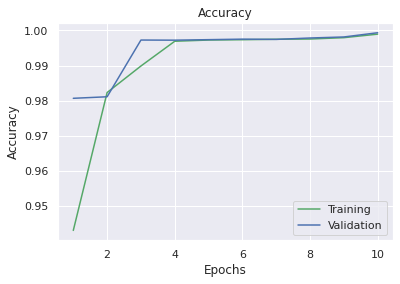
\includegraphics[scale=0.75]{accevo.png}
  \caption{Accuracy Curve for Artificial Neural Network}
\end{figure}

\begin{figure}[H]
  \centering
  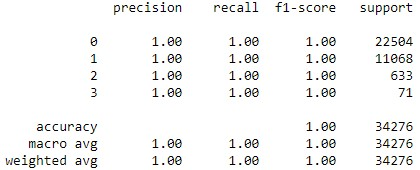
\includegraphics[scale=0.8]{nnreport.jpg}
  \caption{Classification Report for Artificial Neural Network}
\end{figure}

\section{Results}

The accuracies of all models lied was 100\% which means we can accurately predict the severity of an accident. A bar plot is plotted below with the bars representing the accuracy of each model.

\begin{figure}[h]
  \centering
  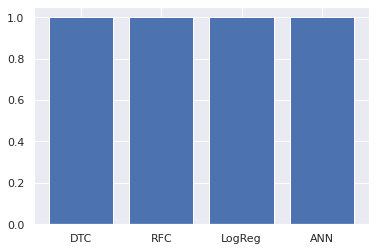
\includegraphics[scale=0.8]{modelcomp.png}
  \caption{Comparison of Model Accuracies}
\end{figure}

\section{Conclusion}

Initially, the classifiers had an prediction accuracy of 66\%-71\%, however, upon going back to the data preparation phase, minor tweaking and taking additional fields in the dataset improved the overall accuracy of all models.

The accuracy of the classifiers is excellent, i.e., 100\%. This means that the model has trained well and fits the training data and performs well on the testing set as well as the training set. We can conclude that this model can accurately predict the severity of car accidents in Seattle.

\section{Future Work}

The trained model can be deployed onto governance and monitoring web and mobile applications to predict the accident severity for a given set of parameters.

\end{document} 